\section{问题二：基于离散制氨调节的运行优化}

\subsection{问题分析}

本问题将制氨产能扩容至72吨/日（设备功率线性翻倍），产量从72吨/日按9吨/日递减至36吨/日共5个水平，电氢氨装置仅有全额开机和停机两种运行方式。需要确定每种产量水平下成本最低的生产时段安排，并在24种风光场景下进行全年统计分析。

\begin{figure}[H]
\centering

\includegraphics[width=0.85\textwidth,height=0.38\textheight,keepaspectratio]{../figures/fig_flow_q2.pdf}
\caption{问题二求解流程图}\label{fig:flow_q2}
\end{figure}

问题二的求解流程如图\ref{fig:flow_q2}所示，核心思路是将连续运行改为选择性开机，通过在风光充足时段集中生产来降低购电成本。由于每个时段的开机决策相互独立（目标函数可分离），可以采用贪心排序算法获得全局最优解。

\subsection{模型建立}

\subsubsection{参数更新}

产能扩容至72吨/日后，设备参数线性翻倍：碱性电解槽$P_{ALK}^{rated} = 20$ MW，PEMEL $P_{PEM}^{rated} = 20$ MW，合成氨装置$P_{NH3}^{rated} = 1.5$ MW，电氢氨总功率$P_{EHA}^{rated} = 41.5$ MW。各产量水平对应的运行时段数为：72吨/日对应24小时，63吨/日对应21小时，54吨/日对应18小时，45吨/日对应15小时，36吨/日对应12小时。

\subsubsection{优化模型}

决策变量为各时段的开停机状态$u(t) \in \{0, 1\}$，$t = 1, 2, ..., 24$。目标函数为最小化吨氨成本：
\begin{equation}\label{eq:q2_obj}
\min \quad C_{ton} = \frac{C_{RE} + C_{OM} + C_{buy} - C_{sell}}{M_{target}}
\end{equation}

约束条件包括产量约束$\sum_{t=1}^{24} u(t) = N_{on}$和功率平衡约束：
\begin{equation}
P_{wind}(t) + P_{pv}(t) + P_{buy}(t) = u(t) \cdot P_{EHA}^{rated} + P_{load}(t) + P_{sell}(t), \quad \forall t
\end{equation}

\subsubsection{贪心排序算法}
考虑到系统缺乏跨时段耦合约束（如储能状态爬坡等），目标函数在时间维度上具备完全可分离性。因此，可将该0-1整数规划转化为针对各独立时段的排序问题。定义时段$t$的开机边际成本$c_t$为：$$c_t = \text{cost}_{ON}(t) - \text{cost}_{OFF}(t)$$其中，$\text{cost}_{ON}(t)$为$t$时段开机时的净运行成本（购电与运维成本之和扣除售电收入），$\text{cost}_{OFF}(t)$为停机时的净成本。将这24个时段的$c_t$升序排列，选取前$N_{on}$个时段赋予状态$u(t)=1$，其余赋予$u(t)=0$，即可在满足产量约束的前提下实现全局最优。

%由于目标函数对各时段可分离，定义每个时段的开机边际成本为$c_t = \text{cost}_{ON}(t) - \text{cost}_{OFF}(t)$，其中$\text{cost}_{ON}(t)$为时段$t$开机时的净成本（购电成本+运维成本-售电收入），$\text{cost}_{OFF}(t)$为停机时的净成本。选择边际成本最低的$N_{on}$个时段开机即为全局最优解。

该算法的最优性可严格证明：设任意可行解$\mathbf{u}$中存在时段$i$开机（$u_i=1$）而时段$j$停机（$u_j=0$），若$c_i > c_j$，则交换$i$和$j$的状态后总成本降低$c_i - c_j > 0$，与最优性矛盾。因此最优解必然选择边际成本最小的$N_{on}$个时段。

\subsection{典型场景求解结果}

\begin{table}[H]
\centering
\caption{典型场景各产量最优方案对比}\label{tab:q2_typical}
\resizebox{\textwidth}{!}{
\begin{tabular}{ccccccc}
\toprule
日产量(吨/日) & 开机时段(h) & 吨氨成本(元/吨) & $R_1$(\%) & $R_2$(\%) & $R_3$(\%) & 达标情况 \\
\midrule
72 & 24 & 6219.14 & 86.52 & 53.26 & 6.74 & 全满足 \\
63 & 21 & 5328.06 & 84.33 & 59.66 & 7.83 & 全满足 \\
54 & 18 & 4591.27 & 80.16 & 67.30 & 9.92 & 全满足 \\
45 & 15 & 3944.54 & 50.98 & 66.67 & 24.51 & 不满足 \\
36 & 12 & 3191.67 & 10.50 & 59.68 & 44.75 & 不满足 \\
\bottomrule
\end{tabular}}
\end{table}

典型场景下各产量水平的最优方案对比如表\ref{tab:q2_typical}所示。吨氨成本随产量降低而单调递减，从72吨/日的6219.14元/吨降至36吨/日的3191.67元/吨，这是因为低产量时可以选择风光最充足的时段集中生产，大幅减少购电需求。吨氨成本最低的日产量为36吨/日（3191.67元/吨），但该产量下$R_1 = 10.50\%$和$R_3 = 44.75\%$均严重不满足绿电指标要求。

绿电指标全满足的最低成本方案为54吨/日（4591.27元/吨），此时$R_1 = 80.16\% > 60\%$，$R_2 = 67.30\% > 30\%$，$R_3 = 9.92\% < 20\%$，三项指标均达标。产量从54吨/日降至45吨/日时，$R_1$从80.16\%骤降至50.98\%，$R_3$从9.92\%跃升至24.51\%，出现了指标的"断崖式"恶化。这是因为45吨/日仅需15小时开机，优化器选择在风光最充足的白天时段集中生产，导致大量风光余电在停机时段上网，推高了$R_3$。

各产量水平的吨氨成本对比和绿电指标雷达图分别如图\ref{fig:q2_cost_compare}和图\ref{fig:q2_indicators}所示。

\begin{figure}[H]
\centering
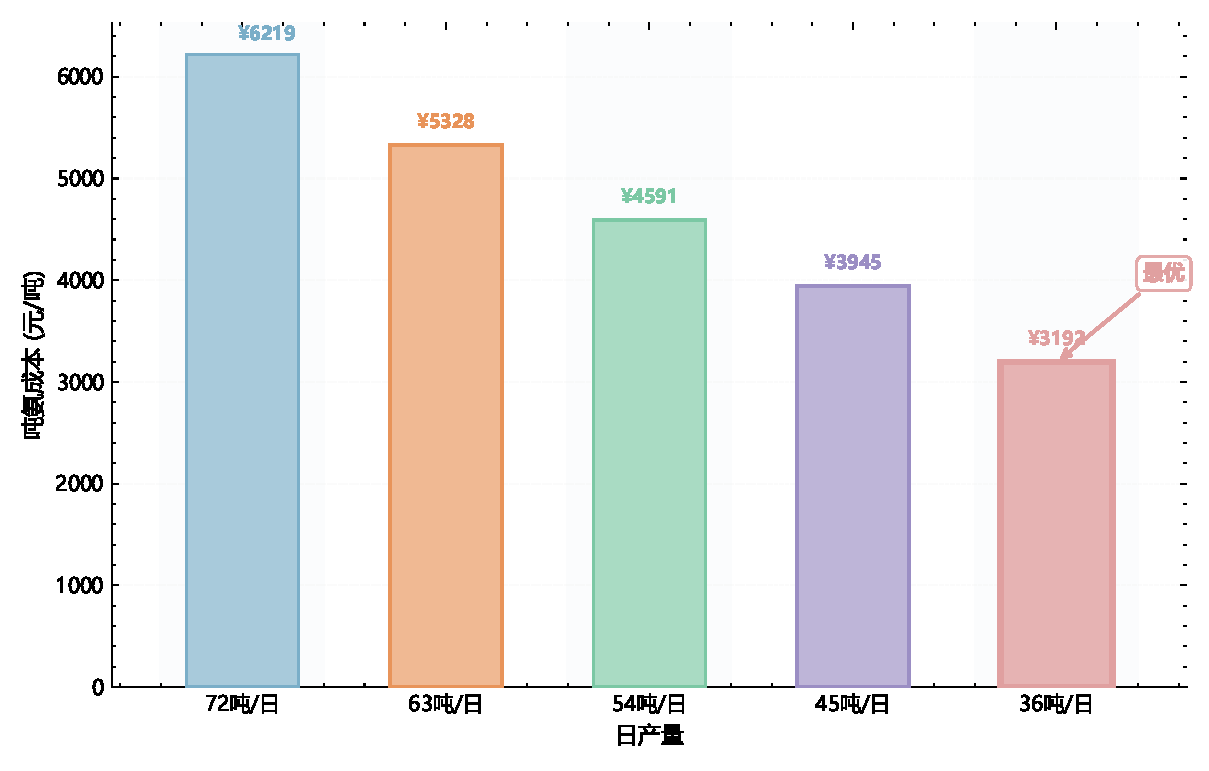
\includegraphics[width=0.85\textwidth,height=0.38\textheight,keepaspectratio]{../figures/fig_q2_cost_compare.pdf}
\caption{不同产量水平的吨氨成本对比}\label{fig:q2_cost_compare}
\end{figure}

成本对比图清晰地展示了产量与成本之间的负相关关系。高产量（72吨/日）需要24小时全开，无法避开电价高峰和风光不足时段，导致大量购电推高成本；低产量（36吨/日）可以精准选择风光充足且电价低谷的时段生产，购电需求大幅降低。但这种"挑时段"策略的代价是绿电指标恶化——停机时段的风光余电全部上网，推高了$R_3$。

\begin{figure}[H]
\centering
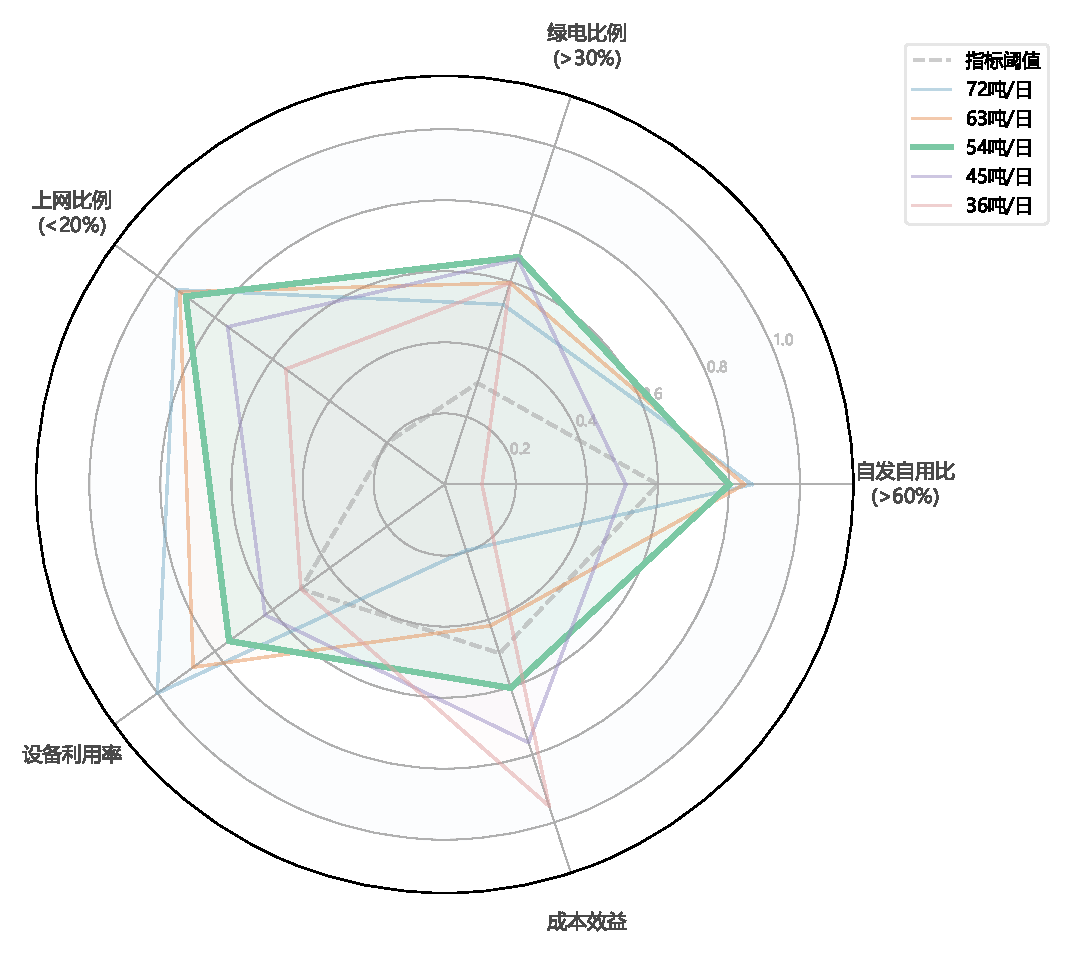
\includegraphics[width=0.85\textwidth,height=0.38\textheight,keepaspectratio]{../figures/fig_q2_indicators.pdf}
\caption{各产量水平绿电指标雷达图对比}\label{fig:q2_indicators}
\end{figure}

雷达图直观地展示了成本与绿电指标之间的权衡关系：高产量方案（72、63、54吨/日）绿电指标优异但成本较高，低产量方案（45、36吨/日）成本低但绿电指标不达标。54吨/日是兼顾经济性和绿电合规的最优平衡点，设备利用率为75\%。

各产量水平的最优开机时段安排如图\ref{fig:q2_gantt}所示。

\begin{figure}[H]
\centering
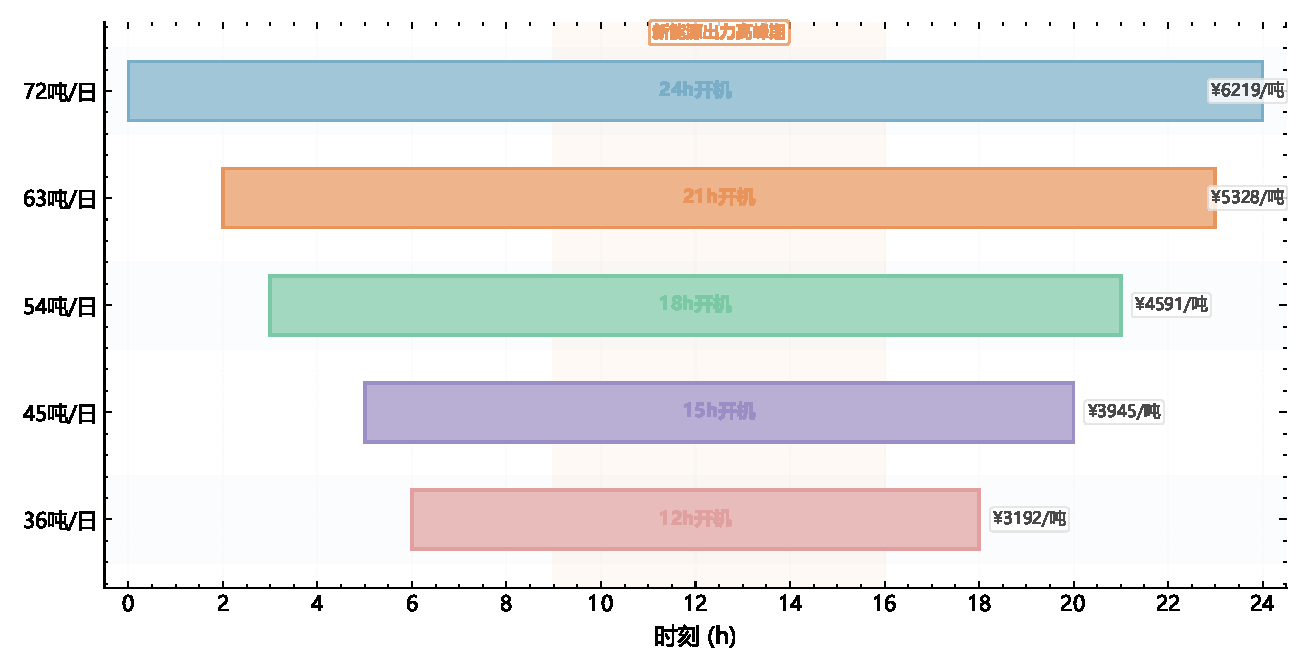
\includegraphics[width=0.85\textwidth,height=0.38\textheight,keepaspectratio]{../figures/fig_q2_gantt.pdf}
\caption{各产量水平最优开机时段安排}\label{fig:q2_gantt}
\end{figure}

从甘特图可以观察到，随着产量降低，停机时段逐渐从夜间向两端扩展。72吨/日全天运行无选择空间；63吨/日停机3小时集中在18:00--20:00（风光最弱时段）；54吨/日停机6小时覆盖17:00--22:00；45吨/日和36吨/日的停机时段进一步扩大到整个夜间。这种模式反映了贪心算法的核心逻辑——优先在风光充足时段开机以最小化购电成本。

\subsection{24种场景全年分析}

对6种风电场景$\times$4种光伏场景=24种组合，每种场景代表15天（24$\times$15=360天$\approx$全年），分别求解各产量水平的最优调度方案。

\begin{figure}[H]
\centering
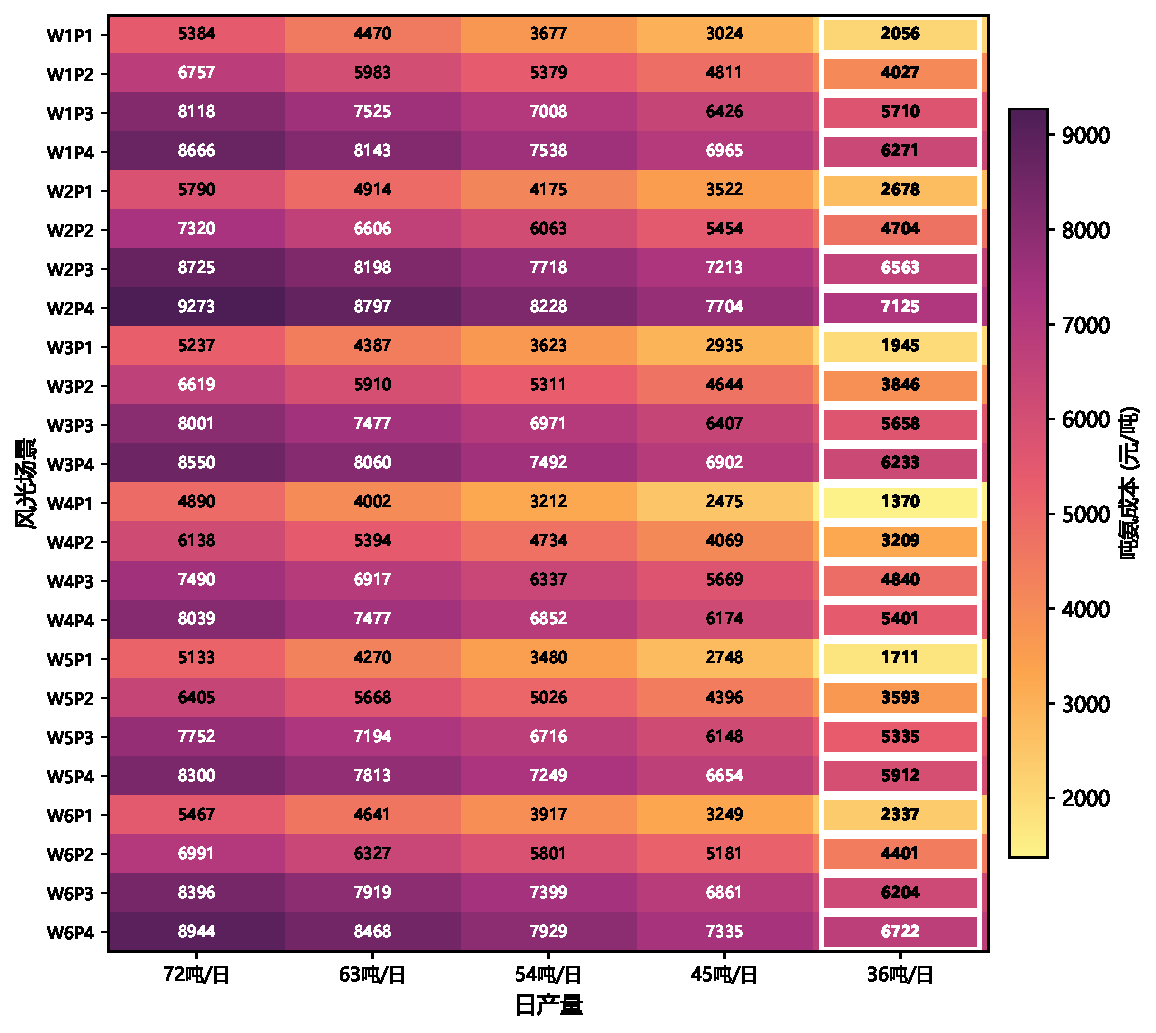
\includegraphics[width=0.85\textwidth,height=0.38\textheight,keepaspectratio]{../figures/fig_q2_scenario_heatmap.pdf}
\caption{24场景$\times$5产量的吨氨成本热力图}\label{fig:q2_scenario_heatmap}
\end{figure}

吨氨成本热力图（图\ref{fig:q2_scenario_heatmap}）揭示了风光资源与成本之间的强相关性。W4P1场景（高风电+高光伏）下各产量成本最低（36吨/日仅1370元/吨），而W2P4场景（中风电+低光伏）下成本最高（72吨/日达9273元/吨）。光伏场景对成本的影响大于风电场景，这与光伏装机容量（64 MW）大于风电装机容量（40 MW）的事实一致。

全年绿电指标统计结果为：全满足场景0个，部分满足场景21个，全不满足场景3个。在所有24种场景下，贪心算法均选择36吨/日作为成本最低产量，但该产量下绿电指标普遍不达标。全不满足的3个场景（W2P3、W2P4、W6P4）对应风光资源较差的组合，此时即使选择最低产量也无法满足$R_2 > 30\%$的要求。

\begin{figure}[H]
\centering
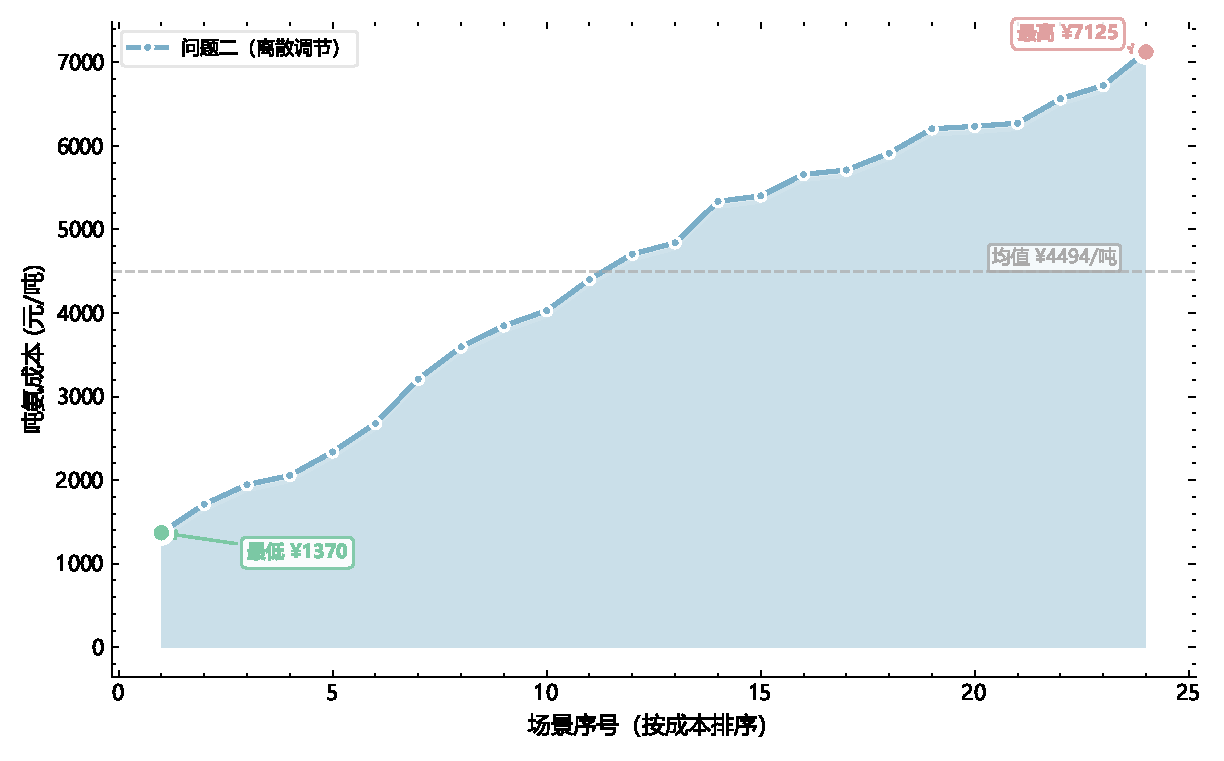
\includegraphics[width=0.85\textwidth,height=0.38\textheight,keepaspectratio]{../figures/fig_q2_annual_cost.pdf}
\caption{全年吨氨成本分布曲线（离散调节）}\label{fig:q2_annual_cost}
\end{figure}

全年吨氨成本分布曲线（图\ref{fig:q2_annual_cost}）呈现明显的右偏分布特征，成本从最低1370元/吨到最高7125元/吨，跨度达5.2倍。全年加权平均吨氨成本为4493.82元/吨。成本分布的离散性反映了风光资源的强随机波动性对园区经济性的显著影响，这也是引入连续调节（问题三）和储能（问题四）的核心动机。
